\documentclass[12pt]{article}
\usepackage[utf8]{inputenc}
\usepackage[margin=0.75in]{geometry}
\usepackage{array}
\usepackage{tabularx}
\usepackage{pifont}
\usepackage{verbatim}
\usepackage{caption}
\usepackage{tikz}
\usetikzlibrary{shapes.geometric}

\tikzstyle{startstop} = [rectangle, rounded corners, minimum width=3cm, minimum height=1cm,text centered, draw=black, fill=red!30]
\tikzstyle{io} = [trapezium, trapezium left angle=70, trapezium right angle=110, minimum width=3cm, minimum height=1cm, text centered, draw=black, fill=blue!30]
\tikzstyle{process} = [rectangle, minimum width=3cm, minimum height=1cm, text centered, draw=black, fill=orange!30]
\tikzstyle{decision} = [diamond, minimum width=3cm, minimum height=1cm, text centered, draw=black, fill=green!30]
\tikzstyle{arrow} = [thick,->,>=stealth]


\title{RISC-V Exceptions and Interrupts}
\author{Sean Keller}
\date{October 2020}

\begin{document}

\maketitle
\newpage

\section{Exception and Interrupt Definitions}
RISC-V defines exceptions as an unusual condition occurring at run time associated with an instruction in the current hart. Exceptions can be organized into six different categories: fetch, load, store, misaligned jump/branch (i.e misaligned instruction address), illegal instruction, and ECALL/EBREAK. Interrupts refer to an external, asynchronous event that may cause the RISC-V hart to experience an unexpected transfer of control. Interrupts are organized into three different categories: external, software, and timer. External interrupts are raised by devices connected to the processor, software interrupts are raised by programs, and timer interrupts are raised when the value in the \emph{xtime} CSR is greater than or equal the value in the \emph{xtimecmp} CSR.

\begin{section}{Exception Handling}
If an exception occurs, control is relinquished by the program that is currently being executed and transferred to the trap handler. The trap handler can be thought of as a set of instructions that the program jumps to and executes before resuming the program at the location that raised the exception. Before an exception can be raised and handled, the trap handler must be initialized. First, the hardware must decide whether it will be handled by the M-mode, S-mode, or U-mode trap handler. By default, all traps are handled by the M-mode trap handler but exceptions raised in S-mode and U-mode can be delegated to the lower-privilege S-mode and U-mode trap handlers respectively through the \emph{medeleg} CSR. The \emph{medeleg} CSR delegates exceptions by raising the bits in positions that correspond to the exception code numbers (more on this later). Next, the hardware writes to the \emph{xtvec} CSR where \emph{x} can be \emph{m}, \emph{s}, or \emph{u} depending on the trap handler the exception is delegated to. The \emph{xtvec} CSR contains a base address and a mode field. This mode field supports two options: direct and vectored\footnote[1]{The only difference between the direct and vectored modes is how they handle interrupts. Direct mode handles interrupts at the base address while the vectored mode handles them at an address that equal to the base address plus four times interrupt cause code}. Regardless of which mode is selected, the trap handler will start at the base address. 

After \emph{medeleg} and \emph{xtvec} are set, the program jumps to the address where the trap handler is located. The first task the trap handler does is to write the \emph{xepc} CSR with the virtual address of the instruction that took the trap. This address is stored so that the program can be returned to and resumed after the trap handler is finished. Next, the xPP field in \emph{mstatus} is written with the two bit privilege level encoding that corresponds to the privilege level the program was in when the exception was raised. In this field, MPP = 10 is M-mode, SPP = 01 is S-mode, and UPP = 00 is U-mode. After xPP is set, the \emph{xtval} CSR is written with exception-specific information. For EBREAKs, misaligned addresses, access faults, and page faults, \emph{mtval} will contain the faulting virtual address. When page-based virtual memory is enabled, \emph{mtval} is written with the faulting virtual address, even for physical-memory access exceptions. For illegal instructions, \emph{mtval} contains the faulting instruction bits of the illegal instruction i.e the faulting instruction. Once this is done, the hardware will write an exception code to the \emph{xcause} CSR. If an instruction raises multiple synchronous exceptions the decreasing priority order of Table 1 indicates which exception is taken and reported in \emph{xcause}. Finally, the trap handler executes an xRET instruction to jump back to the address stored in \emph{xepc} so that the program can resume. This entire process is summarized in Figure 1 with a flow chart.   
\end{section}

\begin{figure}
\centering
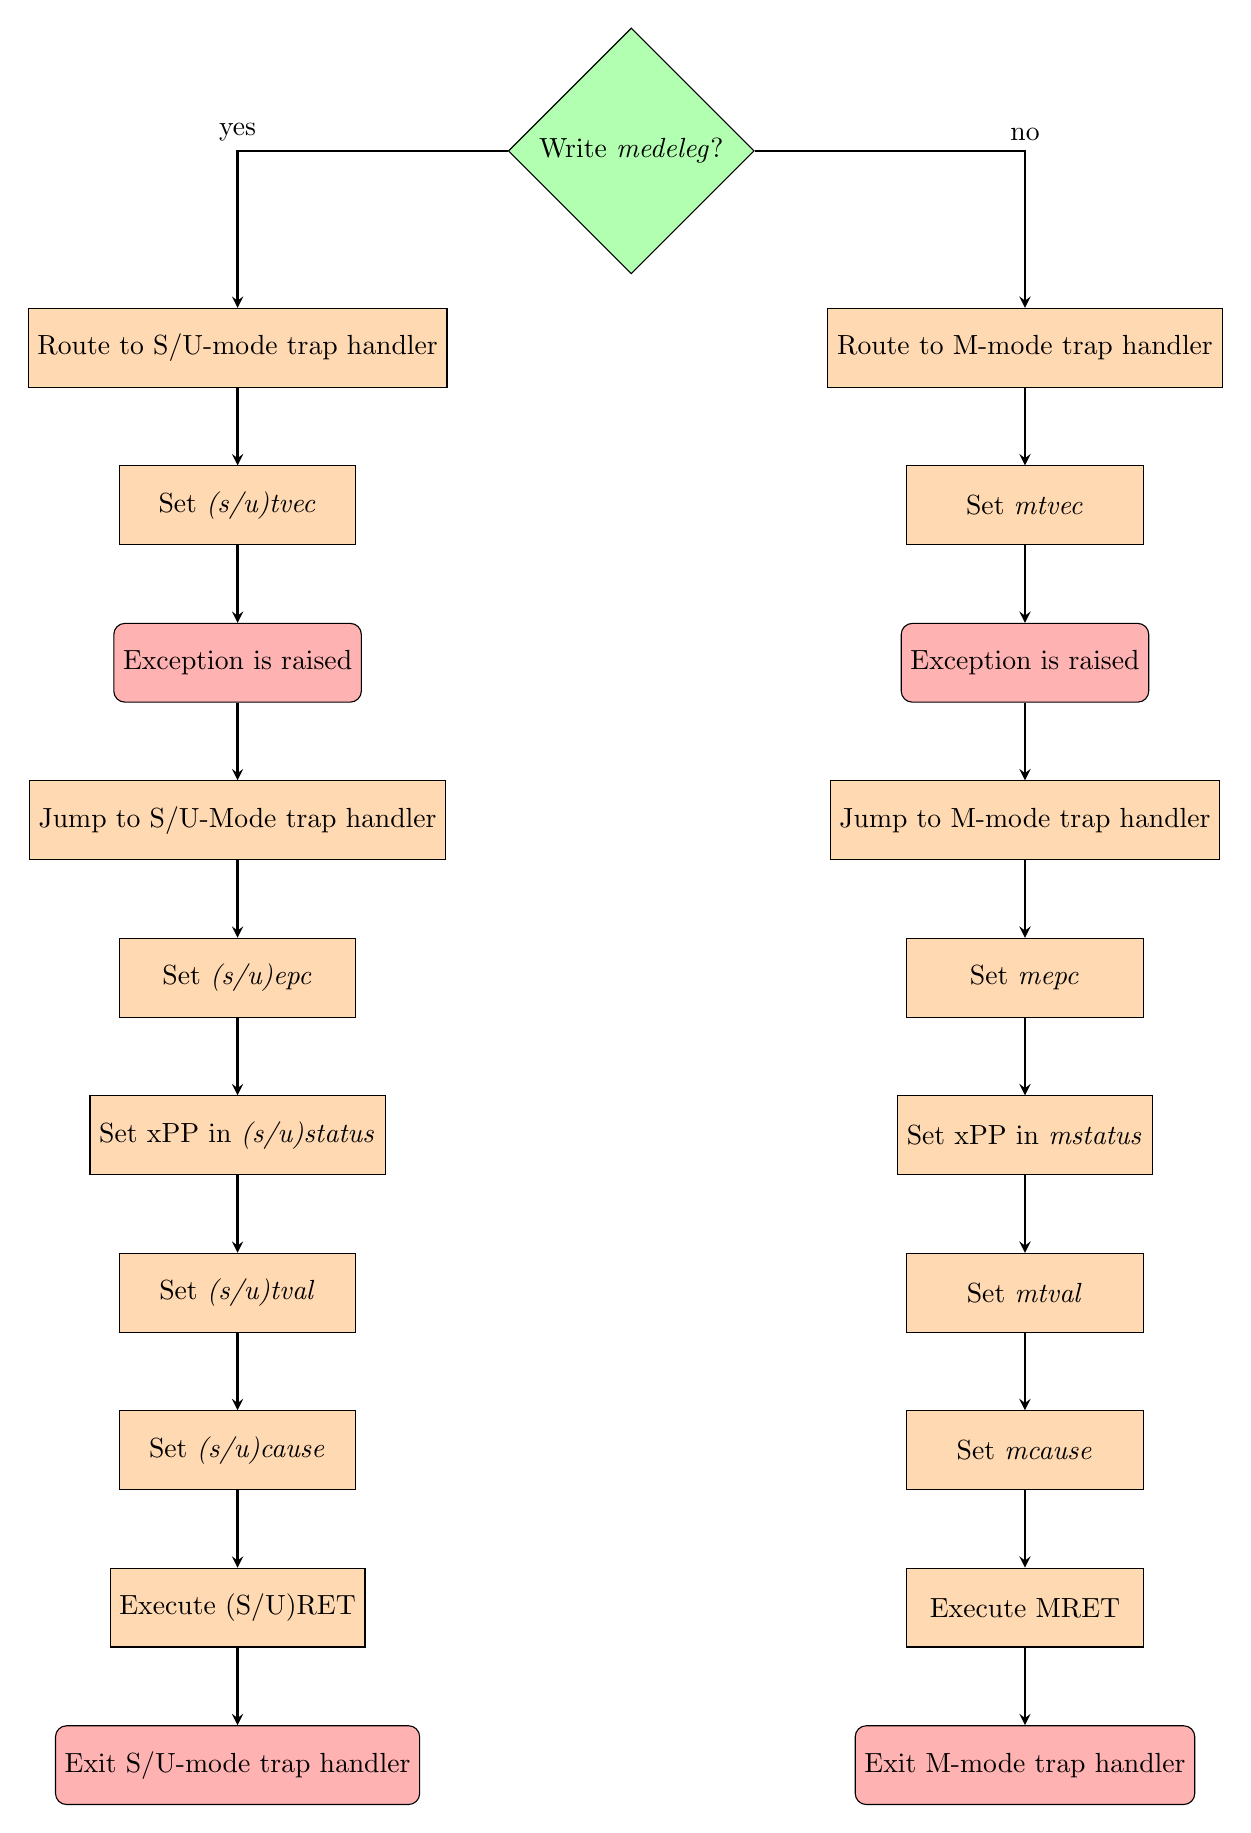
\begin{tikzpicture}[node distance=2cm]
\node (dec1) [decision] {Write \emph{medeleg}?};
\node (pro1a) [process, below of=dec1, xshift=5cm, yshift=-0.5cm] {Route to M-mode trap handler};
\node (pro1b) [process, below of=dec1, xshift=-5cm, yshift=-0.5cm] {Route to S/U-mode trap handler};
\node (pro2a) [process, below of=pro1a] {Set \emph{mtvec}};
\node (pro2b) [process, below of=pro1b] {Set \emph{(s/u)tvec}};
\node (starta) [startstop, below of=pro2a] {Exception is raised};
\node (startb) [startstop, below of=pro2b] {Exception is raised};
\node (pro3a) [process, below of=starta] {Jump to M-mode trap handler};
\node (pro3b) [process, below of=startb] {Jump to S/U-Mode trap handler};
\node (pro4a) [process, below of=pro3a] {Set \emph{mepc}};
\node (pro4b) [process, below of=pro3b] {Set \emph{(s/u)epc}};
\node (pro5a) [process, below of=pro4a] {Set xPP in \emph{mstatus}};
\node (pro5b) [process, below of=pro4b] {Set xPP in \emph{(s/u)status}};
\node (pro6a) [process, below of=pro5a] {Set \emph{mtval}};
\node (pro6b) [process, below of=pro5b] {Set \emph{(s/u)tval}};
\node (pro7a) [process, below of=pro6a] {Set \emph{mcause}};
\node (pro7b) [process, below of=pro6b] {Set \emph{(s/u)cause}};
\node (pro8a) [process, below of=pro7a] {Execute MRET};
\node (pro8b) [process, below of=pro7b] {Execute (S/U)RET};
\node (stopa) [startstop, below of=pro8a] {Exit M-mode trap handler};
\node (stopb) [startstop, below of=pro8b] {Exit S/U-mode trap handler};

\draw [arrow] (dec1) -| node[anchor=south] {no} (pro1a);
\draw [arrow] (dec1) -| node[anchor=south] {yes} (pro1b);
\draw [arrow] (pro1a) -- (pro2a);
\draw [arrow] (pro1b) -- (pro2b);
\draw [arrow] (pro2a) -- (starta);
\draw [arrow] (pro2b) -- (startb);
\draw [arrow] (starta) -- (pro3a);
\draw [arrow] (startb) -- (pro3b);
\draw [arrow] (pro3a) -- (pro4a);
\draw [arrow] (pro3b) -- (pro4b);
\draw [arrow] (pro4a) -- (pro5a);
\draw [arrow] (pro4b) -- (pro5b);
\draw [arrow] (pro5a) -- (pro6a);
\draw [arrow] (pro5b) -- (pro6b);
\draw [arrow] (pro6a) -- (pro7a);
\draw [arrow] (pro6b) -- (pro7b);
\draw [arrow] (pro7a) -- (pro8a);
\draw [arrow] (pro7b) -- (pro8b);
\draw [arrow] (pro8a) -- (stopa);
\draw [arrow] (pro8b) -- (stopb);

\end{tikzpicture}
\caption{Flow Chart of Exception Handling}
\end{figure}

\section{Exception Definitions}
\subsection{Misaligned Addresses}
Misaligned instruction addresses are raised when the target of a jump or branch instruction is not aligned to a 4-byte boundary or an 8-byte boundary. 4-byte alignments are associated with RV32 systems while 8-byte alignments are associated with RV64 systems. 2-byte alignment are also possible for 16-bit instruction implementations but this is a customer instruction encoding. Misaligned loads/store addresses are raised when the data the load/store instruction accesses from memory is not aligned to the correct byte offset. In general, data of size \emph{s} bytes at byte address \emph{A} is aligned if \emph{A} mod \emph{s} = 0.

\subsection{Access Faults}
Instruction, load, and store/AMO access faults are raised from failed physical memory protection checks. Physical memory protection checks verify that the instruction is accessed from a valid address in memory by the hardware. Attempting to fetch an instruction whose physical address lies in a PMP region that does not have execute permissions raises a fetch access exception. Attempting to execute a load or load-reserved instruction whose physical address lies within a PMP region without read permissions raises a load access exception. Attempting to execute a store, store-conditional (regardless of success), or AMO instruction whose physical address lies within a PMP region without write permissions raises a store access exception. Information about execute, read, and write privileges is stored in the lower 3-bits of the page table entry. 

\subsection{Illegal Instructions}
Illegal instructions are raised by illegal instruction encodings or problems reading from and writing to certain CSRs. The following is a non-exhaustive list of illegal instructions that could be raised:
\begin{itemize}
    \item Instructions with bits [15:0] set to zero, this is a reserved bit pattern
    \item Instructions with bits [ILEN-1:0]\footnote[2]{ILEN is the maximum length of the maximum instruction length supported by an implementation. For RISC-V, ILEN is typically 32 or 64 bits.} set to one, this a reserved bit pattern 
    \item Instructions that set rd = x0 with the exception of CSRRW, CSRRWI, JALR, and JAL
    \item Attempts to write to a read-only CSR 
    \item Attempts to access CSRs from non-exsistent CSR addresses
    \item Attempts to access a CSR without appropriate privilege level permissions 
    \item Machine-mode access of machine-level, debug-mode CSRs
    \item Attempts to read or write the satp CSR or execute the SFENCE.VMA instruction while executing in S-mode when the TVM bit in the \emph{xstatus} CSR equals one
    \item Attempts to execute the WFI privilege instruction in any less-privileged mode, and it does not complete within an implementation-specific, bounded time limit\footnote[3]{The time limit may \underline{always} be zero, in which case WFI always causes an illegal instruction exception in less-privileged modes when TW equals one} when the TW bit in the \emph{mstatus} CSR equals one
    \item Attempts to execute SRET while executing in S-mode when the TSR bit in the \emph{xstatus} register equals one
    \item Any instruction that attempts to read or write when the corresponding XS[1:0] field in the \emph{xstatus} CSR is set to zero
    \item Attempts to read to the counter registers that correspond to the IR, TM, and CY bits in the \emph{mcounteren} CSR when executing in a less-privileged mode 
\end{itemize}

\subsection{Environment Call and Environment Break}
The environment call instruction (ECALL) is used to make a request to the supporting execution environment. When executed in U-mode, S-mode, or M-mode, it generates an environment-call-from-U-mode exception, environment-call-from-S-mode exception, or environment-call-from-M-mode exception, respectively, and performs no other operation. ECALL causes the receiving privilege mode’s epc register to be set to the address of the ECALL instruction itself, not the address of the following instruction. On the other hand, the environment break instruction (EBREAK) raises an exception as part of the instruction execution.

\subsection{Page Faults}
For RV32 systems, the supervisor has a 32-bit, page-based virtual memory system called Sv32. RISC-V identifies three different types of page faults: instruction, load, and store/AMO. Instruction page faults are raised by attempting to fetch an instruction from a page that does not have execute permissions. Load page faults are raised by load or load-reserved instructions whose address lies within a page without read permissions. Store/AMO page faults are raised by store, store-conditional, or AMO instruction whose effective address lies within a page without write permissions. In other words, all instructions can raise instruction page faults, load instructions can only raise load page faults, and store instruction can only raise store page faults. This means that load and store page faults also raise instruction page faults. 

The following lists a number of error that can raise a page fault exception that corresponds to the original access type (instruction, load, and store) during the Sv32 virtual to physical address translation process:
\begin{itemize}
    \item The physical address is insufficiently aligned
    \item A virtual page is accessed and the A bit in the PTE is cleared, or is raised and the D bit in the PTE is cleared
    \item PTE bit V = 0, or PTE bit R = 0 and PTE bit W = 1
    \item Performing more than two page walks (i.e i $<$ 0 for i = i - 1 where i = 1 is the first walk and i = 0 is the second walk)
    \item The requested memory access is not allowed by PTE bits R, W, X and U, given the current privlege mode and the value of the SUM and MXR fields in the \emph{mstatus} register
    \item PTE bit A = 0, or if the memory access is a store and PTE bit D = 0
\end{itemize}

\section{Exception Table}
The exceptions in this table fall under the following categories fetch, load, store, misaligned branch/jump, rd != x0 illegal instruction, and ECALL/EBREAK. Fetch exceptions encompass instruction access faults and instruction page faults. Load exceptions encompass misaligned load addresses, load access faults, and load page faults. Store exceptions encompass misaligned store addresses, store access faults, and store page faults. Unless otherwise specified, the fetch, store, and load categories encompass all the respective exceptions included in each category. Misaligned branch/jump exceptions are raised by jump and branch instructions according to the definition for misaligned instruction addresses. EBREAK/ECALL exceptions are raised according to the definitions of environment call and environment break.

\section{Interrupt Handling}
Interrupt handling is similar to exception handling but there are some notable differences. Unlike exceptions, interrupts require additional hardware. This additional hardware includes a Platform Level Interrupt Controller (PLIC) and the option of a SiFive Core-local Interrupter (CLINT) or a RISC-V Core-local Interrupt Controller (CLIC). The PLIC sources external interrupts from devices and sets the interrupt pending bit xEIP bit in the \emph{xip} CSR if it is used with the CLINT. Similarly, the CLINT sources local software and timer interrupts and sets the interrupt pending bits xTIP and xSIP in the \emph{xip} CSR. Unlike the CLINT, the CLIC includes the external interrupt signals from the PLIC and sets the interrupt pending bits xEIP, xTIP, and xSIP. RISC-V has defined a CLIC and PLIC specification\footnote[5]{The CLINT and PLIC specifications are available at https://github.com/riscv/riscv-fast-interrupt/blob/master/clic.adoc and https://github.com/riscv/riscv-plic-spec/blob/master/riscv-plic.adoc respectively. More information about CLINT can be found at https://sifive.cdn.prismic.io/sifive/0d163928-2128-42be-a75a-464df65e04e0\_sifive-interrupt-cookbook.pdf} that explains the interrupt control flow and defines the different registers that are used to handle interrupts. In addition to the CLINT and PLIC, interrupt handling also includes a \emph{xie} CSR that has interrupt enable bits xTIE, xSIE, and xEIE. These bits are set by software and determine when a pending interrupt will be processed through the trap handler. For systems with multiple harts, the Wait for Interrupt (WFI) instruction can be implemented to control interrupt servicing between multiple harts by stalling a hart. If an enabled interrupt is present or later becomes present while the hart is stalled, the interrupt exception will be taken on the following instruction, i.e., execution resumes in the trap handler and \emph{mepc} = pc + 4. The trap handler that is used to process exceptions is the same one that is used to process interrupts. Interrupts processed through this trap handler write to the same CSRs with the exception of \emph{xtvec}. This CSR is only written to when exception are handled by the trap handler.


\begin{center}
\begin{table}
\begin{tabular}{| c || c | c | c | c | c | c |} 
\hline
Instruction & Fetch & Load & Store & Misaligned Branch/Jump & rd != x0 & ECALL/EBREAK \\
\hline
LUI & \ding{53} & & & & \ding{53} & \\
\hline
AUIPC & \ding{53} & & & & \ding{53} & \\
\hline
JAL & \ding{53} & & & \ding{53} & & \\
\hline
JALR & \ding{53} & & & \ding{53} & & \\
\hline
BEQ & \ding{53} & & & \ding{53} & & \\
\hline
BNE & \ding{53} & & & \ding{53} & & \\
\hline
BLT & \ding{53} & & & \ding{53} & & \\
\hline
BGE & \ding{53} & & & \ding{53} & & \\
\hline
BLTU & \ding{53} & & & \ding{53} & & \\
\hline
BGEU & \ding{53} & & & \ding{53} & & \\
\hline
LB & \ding{53} & \ding{53} & & & \ding{53} & \\
\hline
LH & \ding{53} & \ding{53} & & & \ding{53} & \\
\hline
LW & \ding{53} & \ding{53} & & & \ding{53} & \\
\hline
LBU & \ding{53} & \ding{53} & & & \ding{53} & \\
\hline
LHU & \ding{53} & \ding{53} & & & \ding{53} & \\
\hline
SB & \ding{53} & & \ding{53} & & & \\
\hline
SH & \ding{53} & & \ding{53} & & & \\
\hline
SW & \ding{53} & & \ding{53} & & & \\
\hline
ADDI & \ding{53} & & & & \ding{53} & \\
\hline
SLTI & \ding{53} & & & & \ding{53} & \\
\hline
SLTIU & \ding{53} & & & & \ding{53} & \\
\hline
XORI & \ding{53} & & & & \ding{53} & \\
\hline
ORI & \ding{53} & & & & \ding{53} & \\
\hline
ANDI & \ding{53} & & & & \ding{53} & \\
\hline
SLLI & \ding{53} & & & & \ding{53} & \\
\hline
SRLI & \ding{53} & & & & \ding{53} & \\
\hline
SRAI & \ding{53} & & & & \ding{53} & \\
\hline
ADD & \ding{53} & & & & \ding{53} & \\
\hline
SUB & \ding{53} & & & & \ding{53} & \\
\hline
SLL & \ding{53} & & & & \ding{53} & \\
\hline
SLT & \ding{53} & & & & \ding{53} & \\
\hline
SLTU & \ding{53} & & & & \ding{53} & \\
\hline
XOR & \ding{53} & & & & \ding{53} & \\
\hline
SRL & \ding{53} & & & & \ding{53} & \\
\hline
SRA & \ding{53} & & & & \ding{53} & \\
\hline
OR & \ding{53} & & & & \ding{53} & \\
\hline
AND & \ding{53} & & & & \ding{53} & \\
\hline
ECALL & \ding{53} & & & & \ding{53} & \ding{53} \\
\hline
EBREAK & \ding{53} & & & & \ding{53} & \ding{53} \\
\hline
\end{tabular}
\caption{Possible Exceptions for RV32I Instruction Set}
\end{table}
\end{center}
\end{document}